% !TEX root = ../thesis.tex

\chapter{Materials and Methodology}\label{ch:methodology}

\section{Overview of the Proposed Workflow}

The methodology of this thesis is designed as a reproducible workflow for binary semantic segmentation of archaeological features in LiDAR-derived raster data. The workflow connects the available geospatial data, reference annotations, input raster representations, dataset construction, model training, inference, and GIS-based interpretation into a single experimental pipeline.

The proposed workflow consists of the following main stages. First, the available LiDAR-derived data from Guatemala and Slovakia are described and prepared for further processing. Second, the reference annotations are converted into raster masks suitable for pixel-wise supervised learning. Third, several input representations are prepared from the available terrain data and used as alternative inputs for segmentation models. Fourth, the raster data and masks are divided into tiles and organized into training, validation, and testing subsets. Fifth, segmentation models are trained under controlled experimental settings. Finally, the trained models are applied to larger raster areas, and their predictions are exported for quantitative evaluation and qualitative GIS-based assessment.

This chapter describes the materials and methodological decisions used to construct the workflow. The detailed experimental comparison of individual configurations, including the evaluation metrics and experiment groups, is provided separately in Chapter~\ref{ch:design_protocol}.

\section{Study Areas and Data Sources}

Two LiDAR datasets are used in this thesis. They provide two distinct archaeological and geographical contexts for evaluating the proposed segmentation workflow. The first dataset represents Maya archaeological structures in the tropical lowlands of Guatemala, while the second dataset represents terrace-like archaeological features in the Slovak landscape.

The use of both datasets is important for two reasons. First, they allow the methodology to be evaluated on different types of archaeological objects: compact polygonal structures in the Maya dataset and elongated terrace features in the Slovak dataset. Second, their differences in spatial resolution, morphology, and annotation type make it possible to assess how stable the proposed workflow remains when applied to a different data domain.

\subsection{Maya LiDAR Data}

The Maya LiDAR dataset is one of the central data sources used in this thesis. It originates from the Pacunam LiDAR Initiative (PLI), which conducted a large-scale airborne LiDAR survey of the Maya Biosphere Reserve in the department of Petén, Guatemala, in 2016. Within this broader survey, the area around the ancient city of Uaxactun, corresponding to the PARU\footnote{Proyecto Arqueológico Regional Uaxactún} research zone, is used as the primary Maya study area.

The area was scanned using a Teledyne Optech Titan MW airborne laser scanner from an altitude of approximately 650~m above ground level. The scanner was designed to produce a nominal pulse density of 15 pulses per square metre. However, due to dense tropical vegetation, the average ground return density varied approximately between 1.1 and 5.3 returns per square metre~\cite{bundzel_semantic_2020}. The available raster data are represented as a bare-earth Digital Elevation Model (DEM) with a spatial resolution of 1~m per pixel.

The archaeological interpretation of the Uaxactun area was carried out by PARU experts. The structures were identified by visual interpretation of LiDAR-derived terrain products and by using archaeological domain knowledge and field experience. The resulting reference data were stored as georeferenced vector polygons in a GIS environment. The annotations were also verified to a large extent through fieldwork. According to Bundzel et al.~\cite{bundzel_semantic_2020}, the available field validation suggests that the identifications are accurate but slightly conservative, and that field verification revealed approximately 15\% more structures than were visible in the LiDAR-based interpretation.

The original annotation distinguishes two main groups of archaeological objects:
\begin{enumerate}
    \item \textbf{Structures} --- areas of ancient construction activity, including buildings and the platforms on which buildings were constructed.
    \item \textbf{Mounds} --- remains of former buildings without the surrounding platforms.
\end{enumerate}

In this thesis, the Maya data are used for the segmentation of annotated archaeological objects, combining structures and mounds visible in the LiDAR-derived terrain representation. In addition to the previously annotated Uaxactun research polygon, a larger LiDAR coverage is available for contextual visualization and potential inference outside the originally used training and validation areas but provides only elevation data, without any annotations.

\begin{figure}[h]
	\centering
	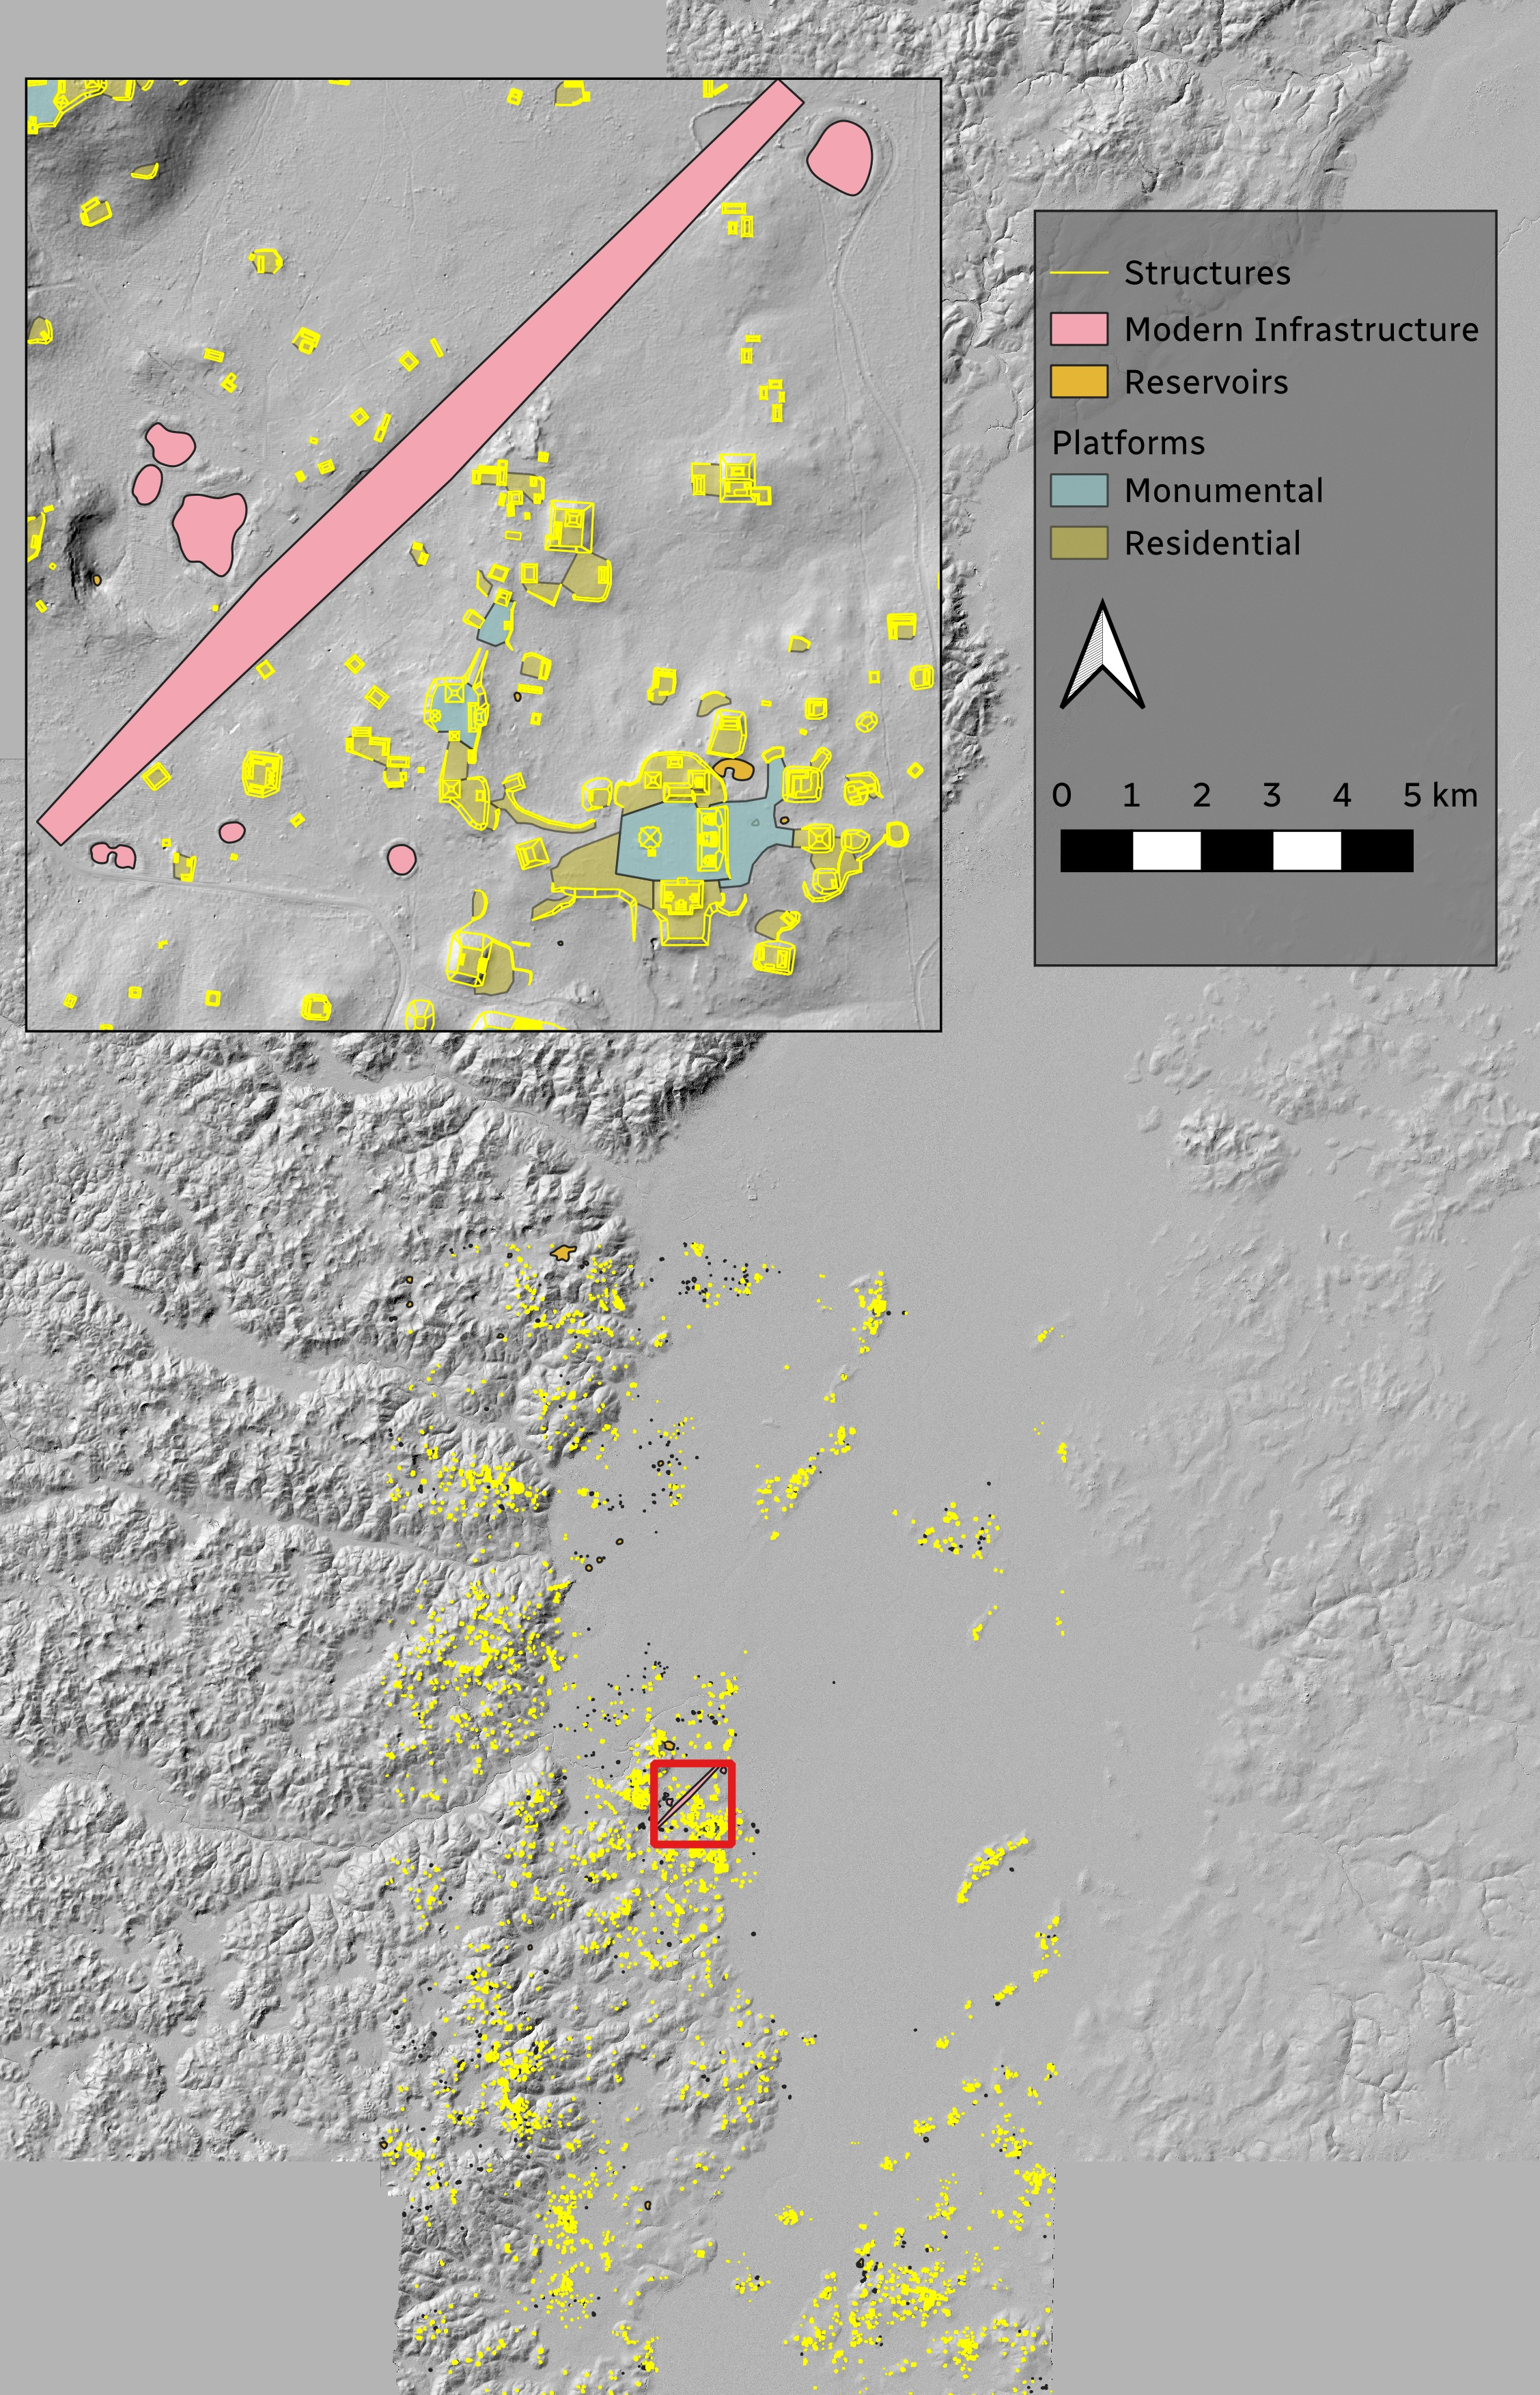
\includegraphics[width=\textwidth]{figures/DEM21_Full_Map.jpg}
	\caption{Overview of the available Maya LiDAR data used in the research.}
	\label{fig:maya_map_overview}
\end{figure}

The spatial extent of the Maya LiDAR data used in this thesis is shown in Figure~\ref{fig:maya_map_overview}. For descriptive analysis, the annotated archaeological structures were divided into three size categories:
\begin{itemize}
    \item \textbf{Small structures} --- structures covering less than 50~m\textsuperscript{2}.
    \item \textbf{Medium-sized structures} --- structures covering between 50 and 200~m\textsuperscript{2}.
    \item \textbf{Large structures} --- complex structures covering more than 200~m\textsuperscript{2}, often formed by platforms and associated construction remains.
\end{itemize}

\begin{figure}[htbp]
	\centering
	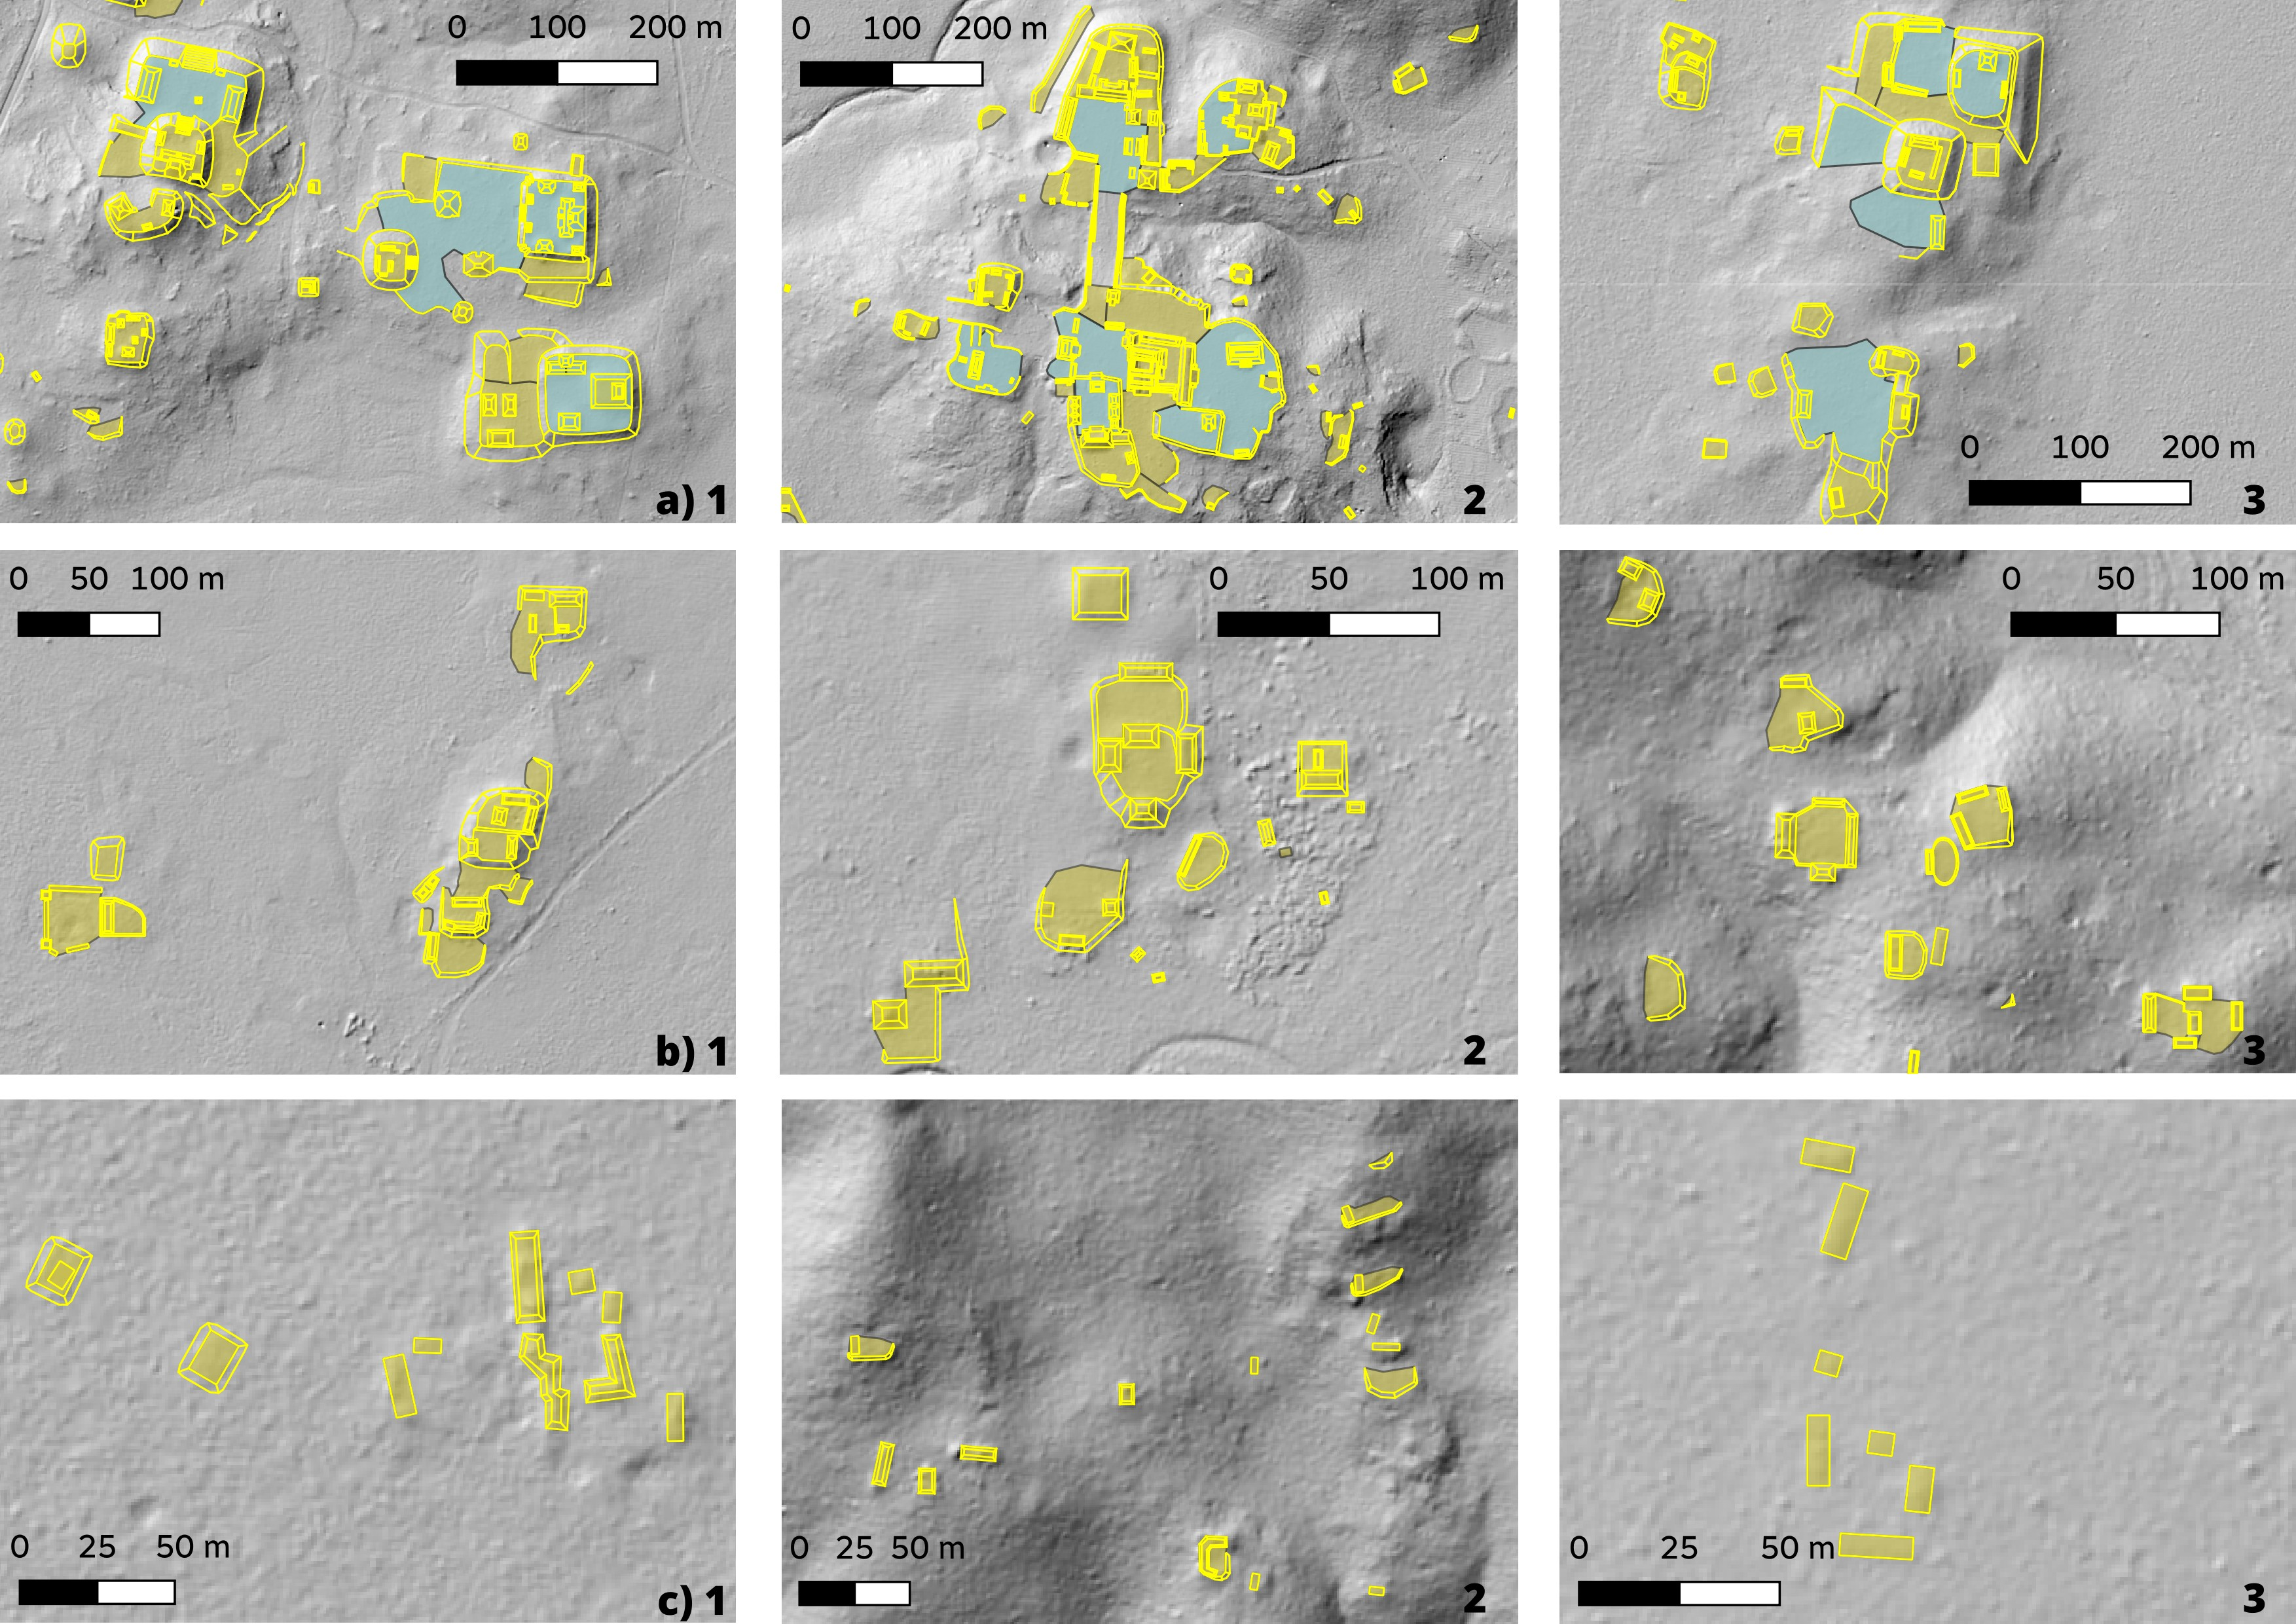
\includegraphics[width=\textwidth]{figures/Maya_Big_Medium_Small_Buildings.jpg}
	\caption{Examples of Maya structures by size category: a) large structures (\textgreater{}200~m\textsuperscript{2}), b) medium-sized structures (50--200~m\textsuperscript{2}), and c) small structures (\textless{}50~m\textsuperscript{2}).}
	\label{fig:maya_structures_visualization}
\end{figure}

\begin{table}[htbp]
\centering
\begin{tabular}{lrrrr}
\hline
Size category & Count & Total area (m\textsuperscript{2}) & Objects (\%) & Map area (\%) \\ \hline
Small  & 1491 & 47756  & 36.15 & 0.028537 \\
Medium & 2164 & 211519 & 52.47 & 0.126395 \\
Large  & 469  & 192608 & 11.37 & 0.115094 \\ \hline
\end{tabular}
\caption{Distribution of Maya archaeological structures by size category and their coverage within the mapped area.}
\label{tab:maya_structures_size}
\end{table}

\begin{figure}[htbp]
	\centering
	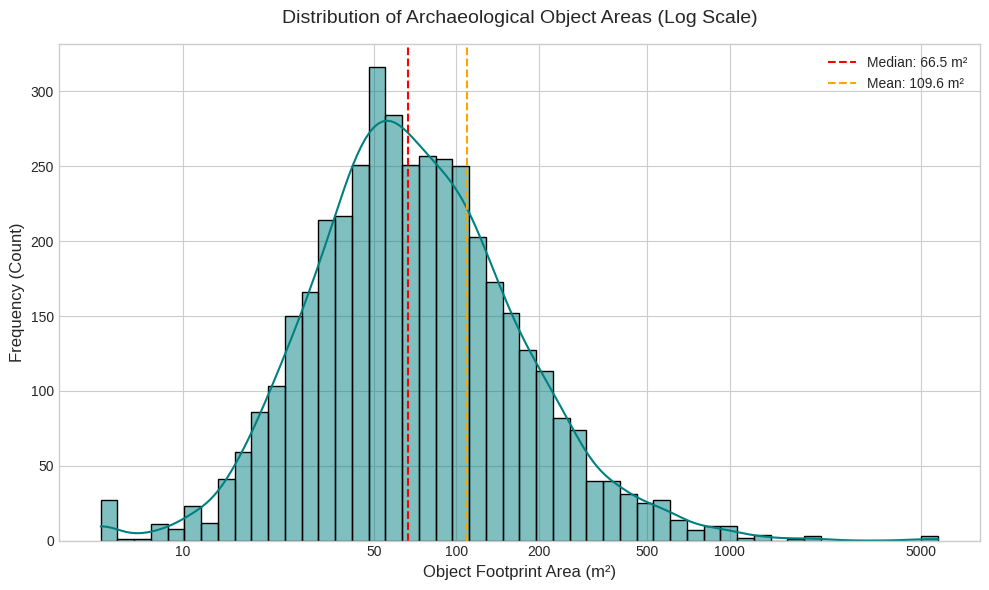
\includegraphics[width=\textwidth]{figures/maya_objects_distribution.png}
	\caption{Distribution of Maya archaeological structures by size category within the mapped area.}
	\label{fig:maya_structures_histogram}
\end{figure}

Figure~\ref{fig:maya_structures_visualization} illustrates the visual appearance of structures from the three size categories. In total, 4,124 structures were identified in the mapped area. Their distribution is summarized in Table~\ref{tab:maya_structures_size} and visualized in Figure~\ref{fig:maya_structures_histogram}. Medium-sized structures form the largest group, representing slightly more than half of all annotated objects.

\subsection{Slovak LiDAR Data}

The Slovak LiDAR data used in this thesis were provided by the Slovak University of Technology in Bratislava, Faculty of Civil Engineering (STU, StF), in cooperation with the Department of Archaeology of the Monuments Board of the Slovak Republic. This dataset represents a second, independent geographical and archaeological context, complementing the Maya data from Guatemala. While the Guatemalan data focus mainly on ancient Maya buildings and construction activity, the Slovak data are oriented toward the detection of archaeological terrace systems in Central European terrain.

The Slovak dataset contains four locations: Ladzany, Sitno, \v{S}\'{a}\v{s}ovsk\'{e} Podhradie, and Tribe\v{c}. All locations except Tribe\v{c} include reference annotations in the form of vector polylines representing the central lines of terraces. The raster resolution is 0.25~m per pixel, which is four times finer in linear resolution than the 1~m Maya DEM. This higher resolution is important for terrace detection, because terraces are narrow and elongated micro-relief structures whose visibility may be strongly affected by the spatial resolution of the raster data.

\begin{figure}[p]
    \centering

    \begin{minipage}[c][0.76\textheight][c]{0.39\textwidth}
        \centering
        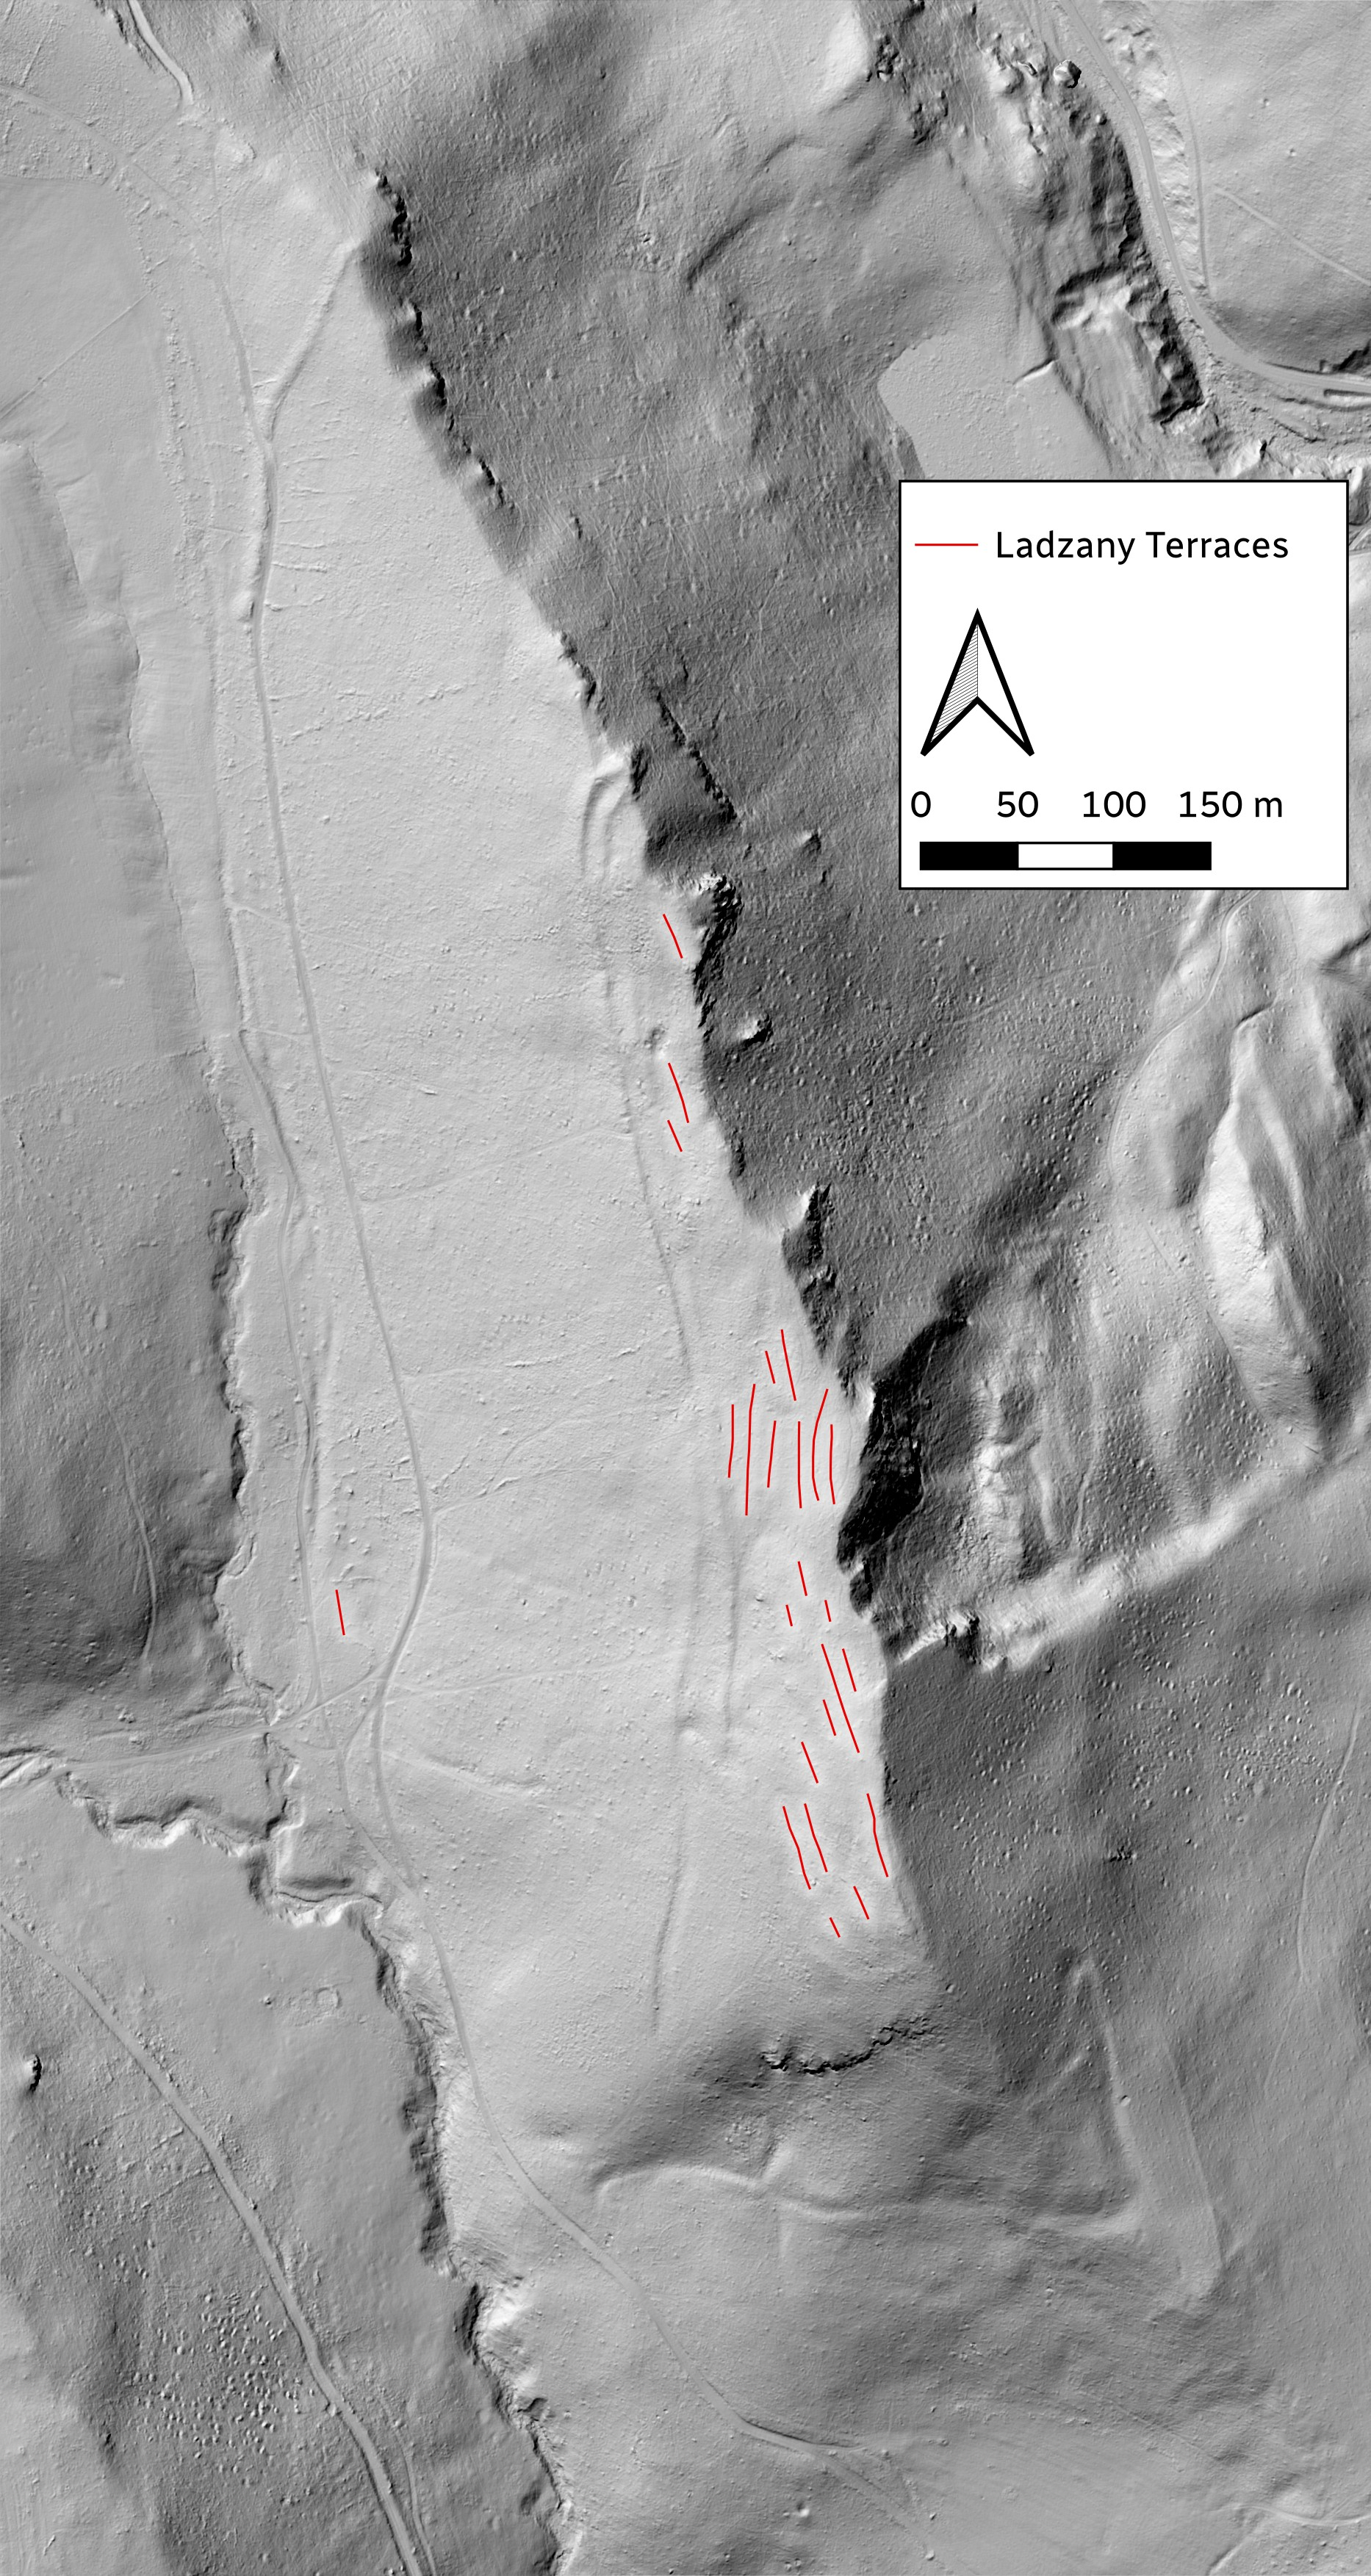
\includegraphics[
            width=\linewidth,
            height=0.62\textheight,
            keepaspectratio
        ]{figures/Ladzany_Full_Map.jpg}
    \end{minipage}
    \hspace{4mm}
    \begin{minipage}[c][0.76\textheight][c]{0.52\textwidth}
        \centering
        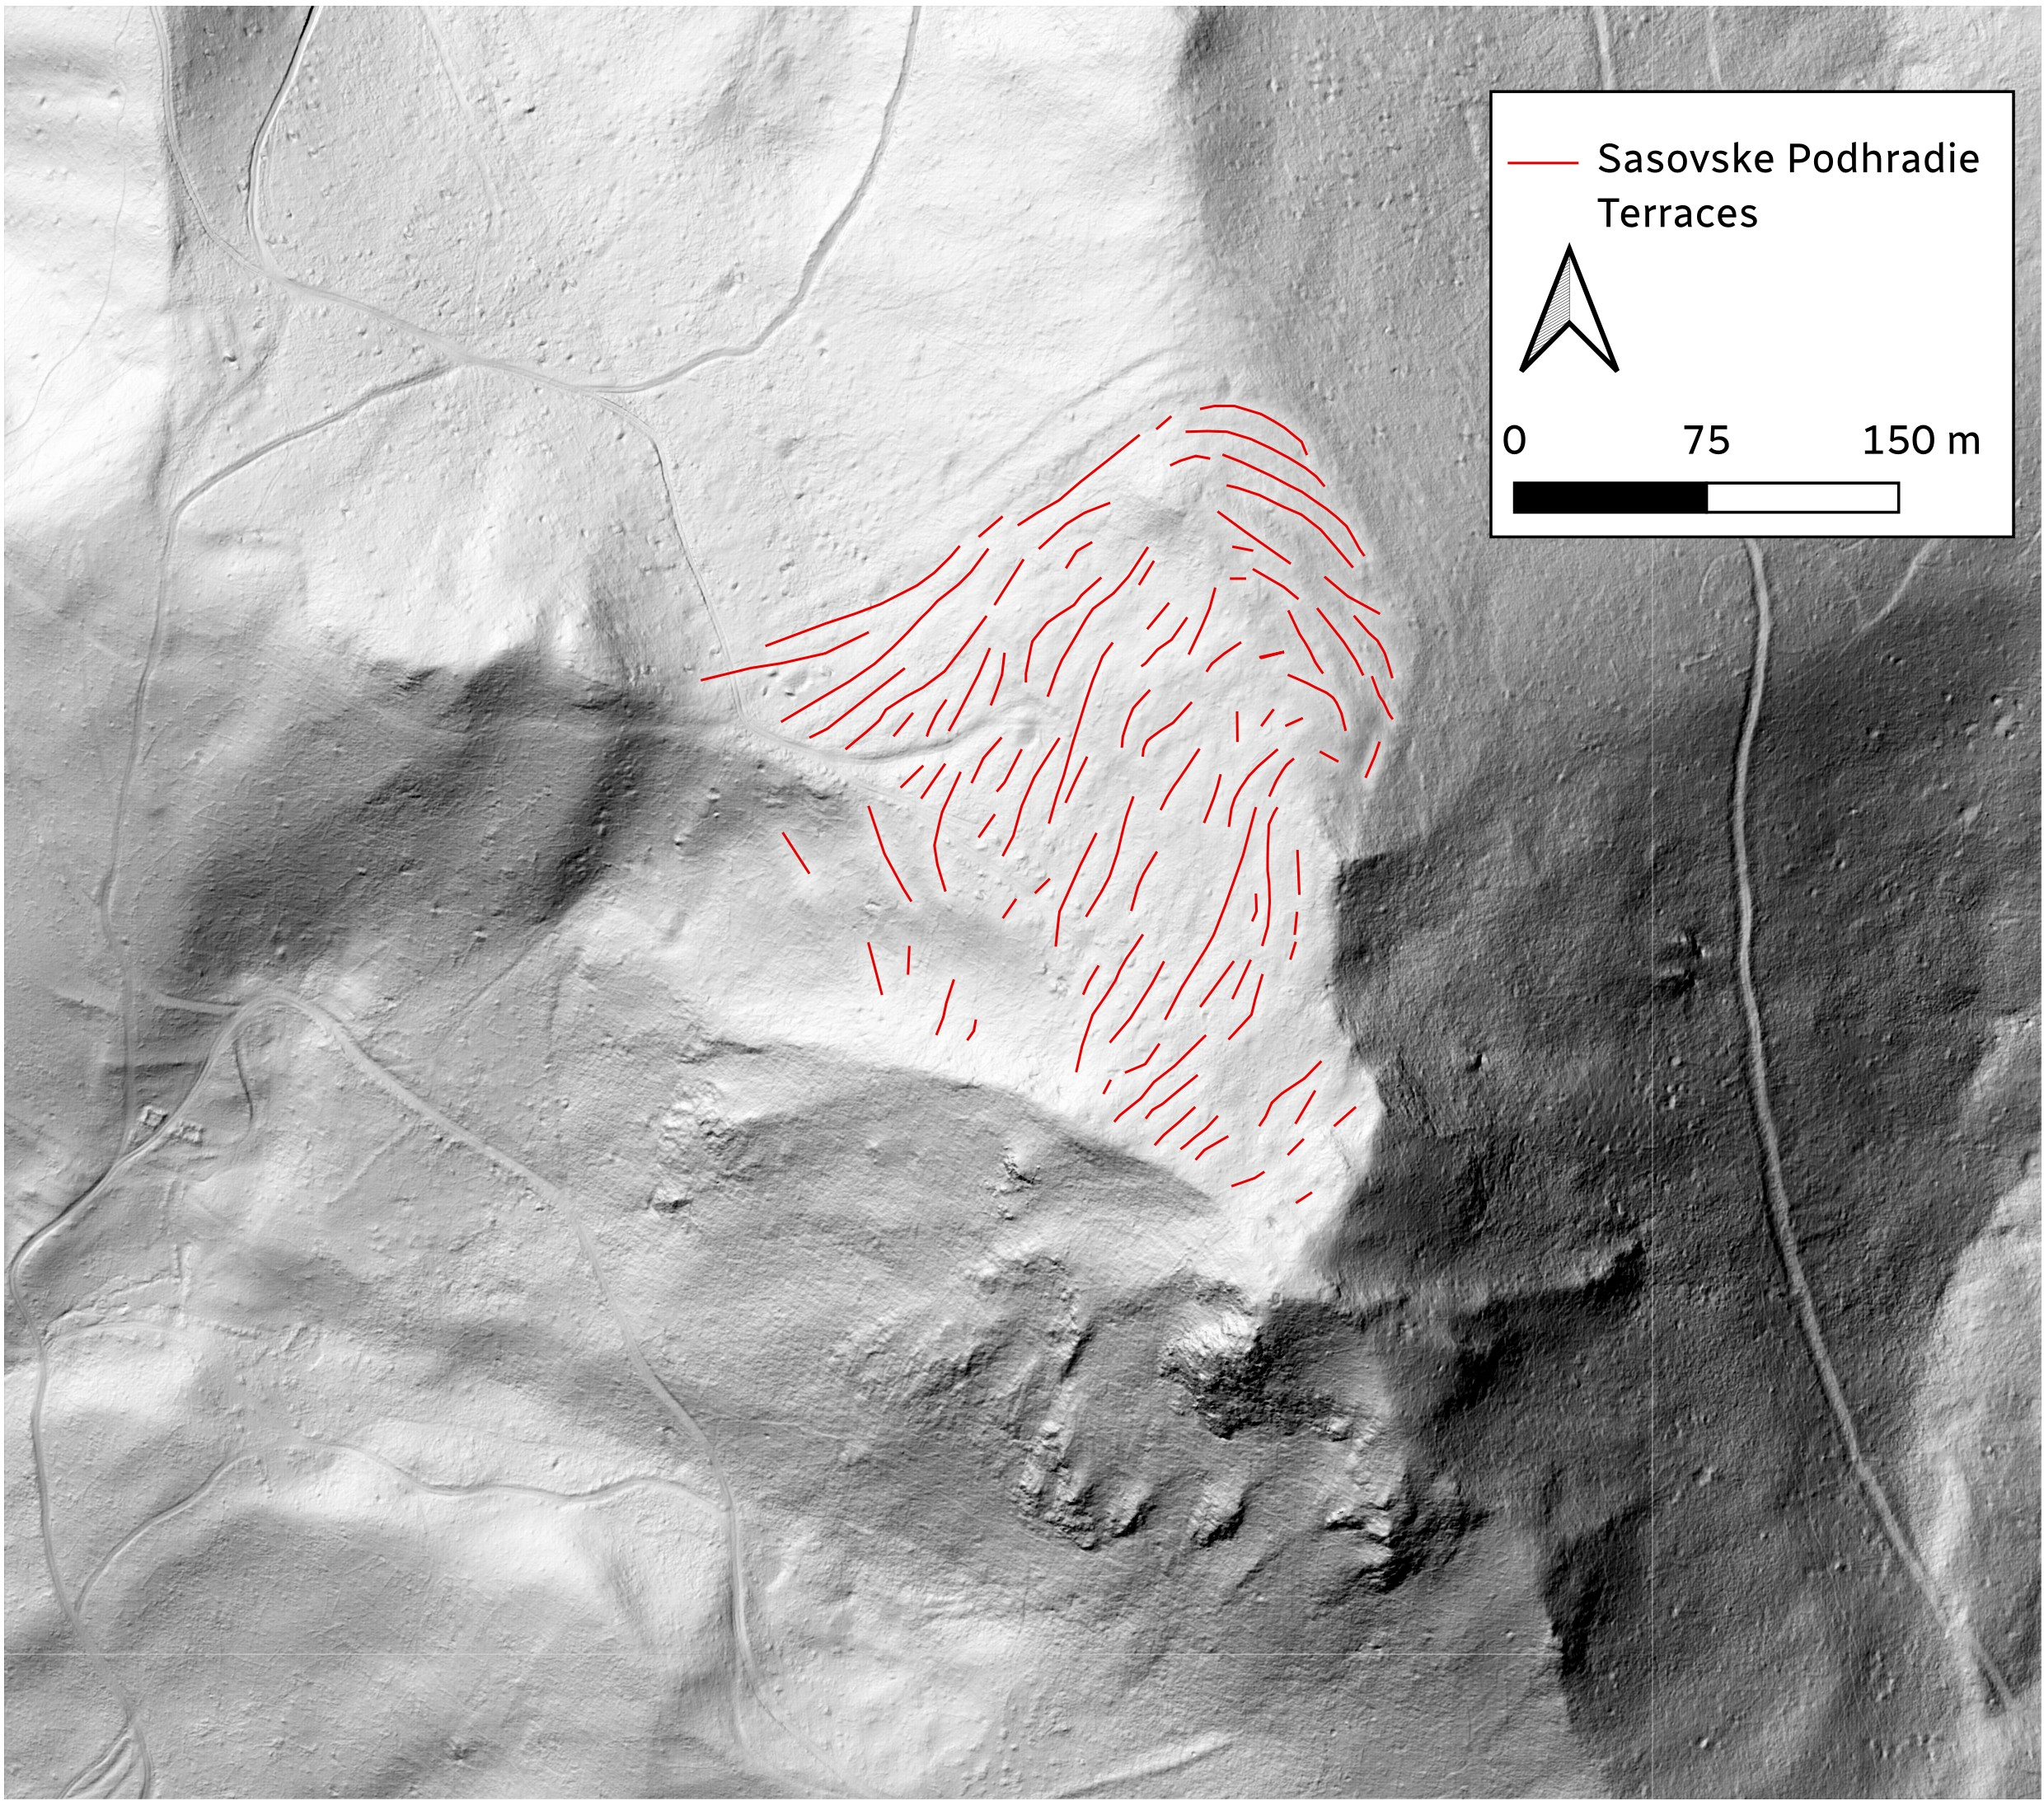
\includegraphics[
            width=\linewidth,
            height=0.22\textheight,
            keepaspectratio
        ]{figures/Sasovske_Full_Map.jpg}

        \vspace{2mm}

        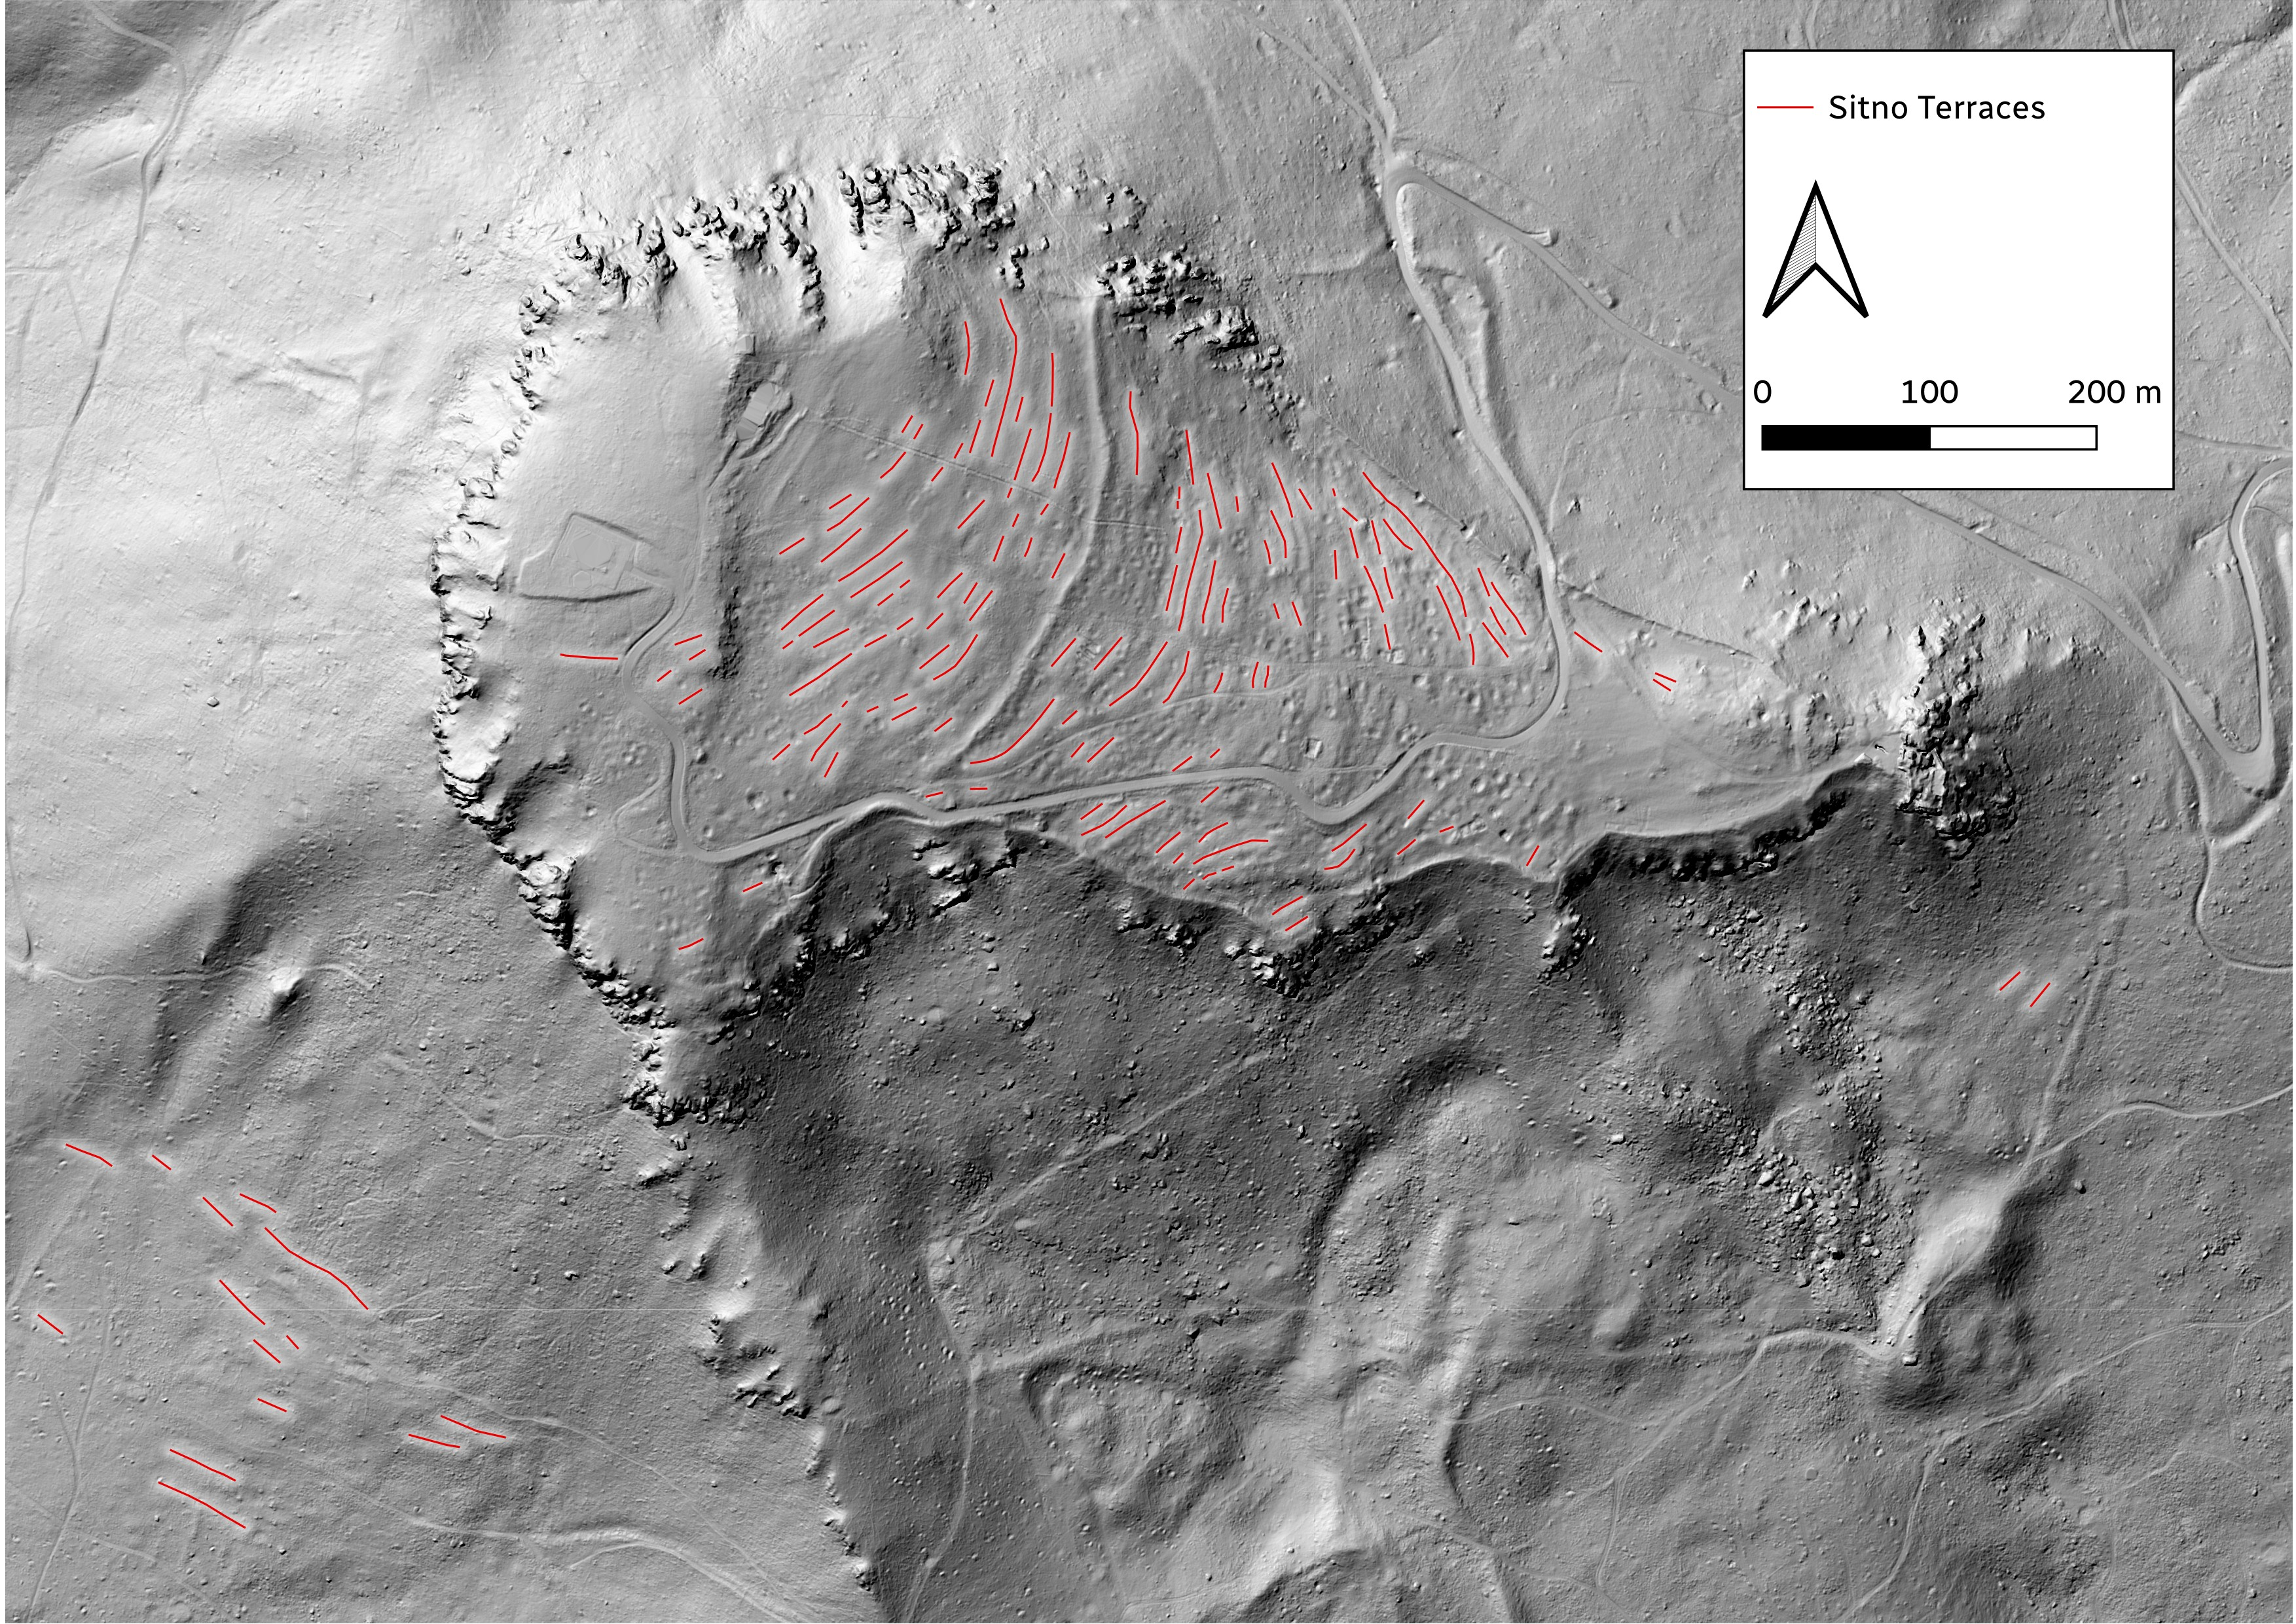
\includegraphics[
            width=\linewidth,
            height=0.22\textheight,
            keepaspectratio
        ]{figures/Sitno_Full_Map.jpg}

        \vspace{2mm}

        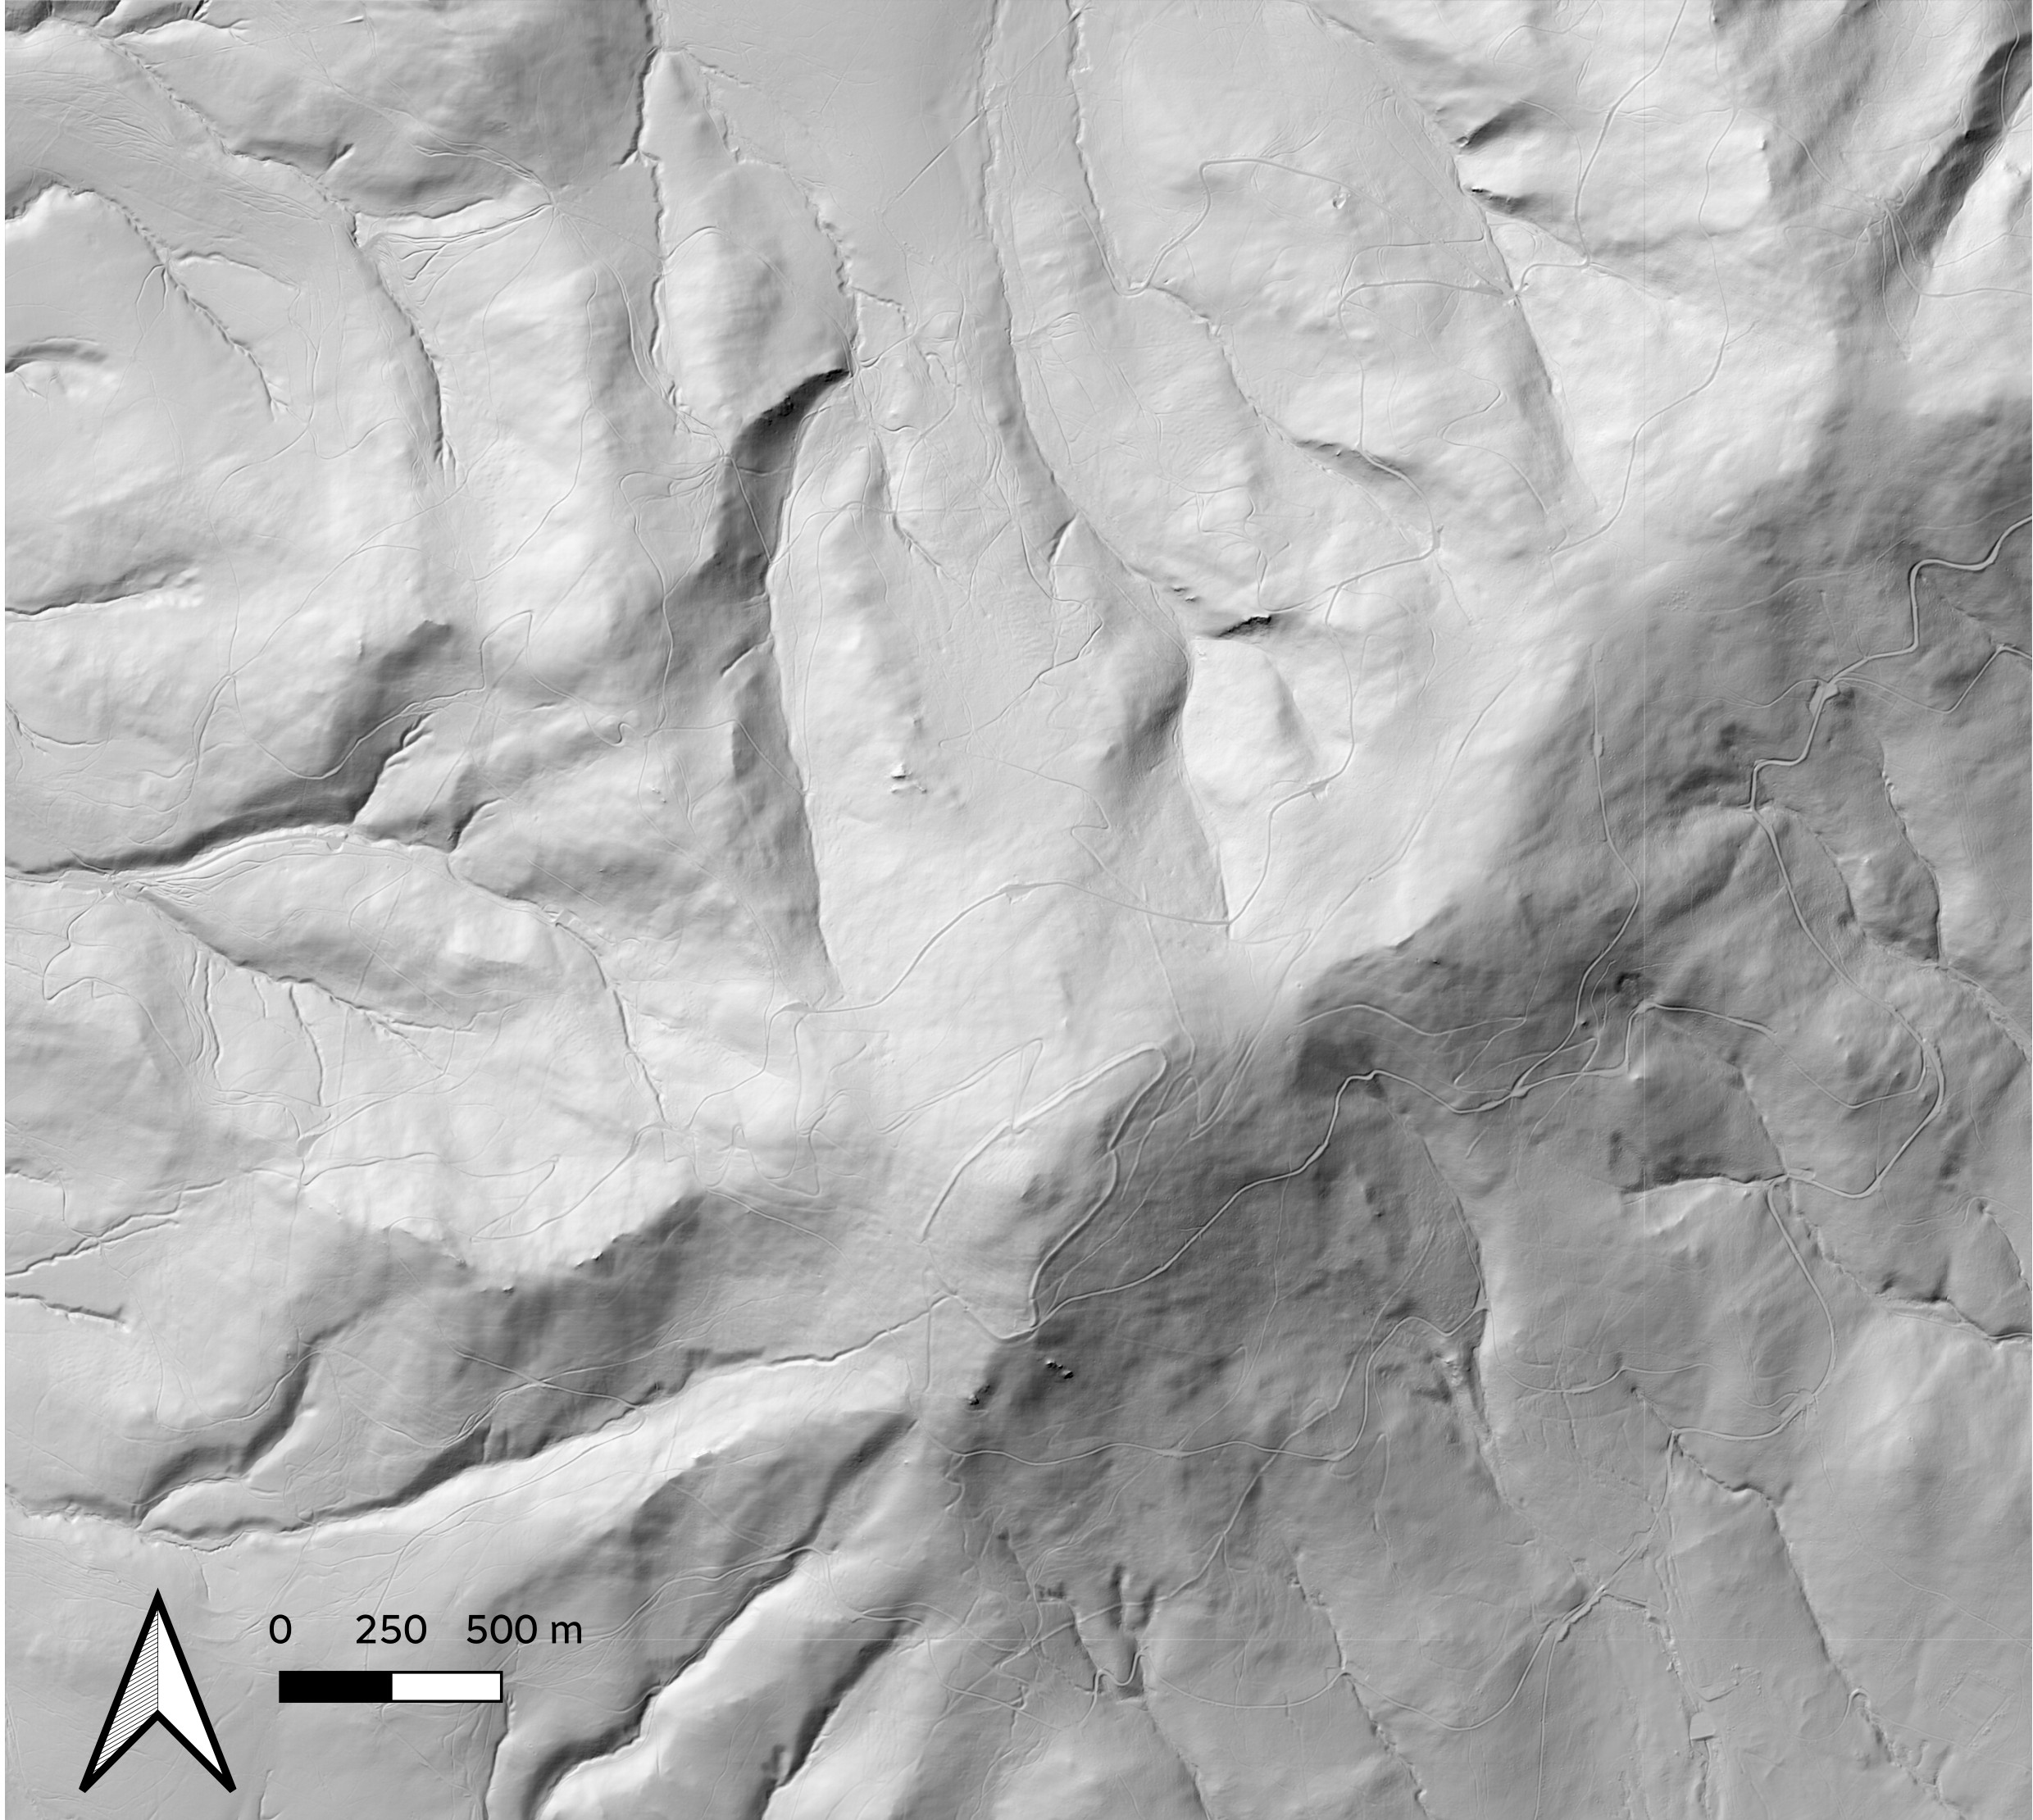
\includegraphics[
            width=\linewidth,
            height=0.22\textheight,
            keepaspectratio
        ]{figures/Tribec_Full_Map.jpg}
    \end{minipage}

    \caption{Overview of the available Slovak LiDAR datasets used in the research.}
    \label{fig:slovak_lidar_data_views}
\end{figure}

\section{Reference Data and Label Preparation}

The preparation of reference annotations has a direct influence on the quality of semantic segmentation and on the stability of model training. Archaeological annotations are not always equivalent to exact machine-learning ground truth. They are produced through expert interpretation and can therefore contain uncertainty, conservative boundaries, simplified geometry, or systematic bias. In the case of LiDAR archaeology, this problem is especially important because the model is trained on the relationship between a rasterized terrain representation and the corresponding annotation mask.

A known issue in the Maya dataset is the so-called \textit{malerization}, where LiDAR-visible archaeological structures are redrawn into schematic forms that represent their interpreted shape, size, and height. This process is useful for archaeological documentation, but it may introduce a mismatch between the idealized representation of a former structure and the actual dispersed micro-relief visible in the present terrain model~\cite{bundzel_semantic_2020}. As a result, the segmentation model may learn not only archaeological morphology, but also the conventions and imperfections of the annotation process.

\subsection{Maya Reference Masks}

For the Maya dataset, the original vector annotations were converted into raster masks aligned with the DEM grid. Two types of binary masks are available in the original methodology: the \textit{Structures} mask, containing buildings and platforms, and the \textit{Mounds} mask, containing building remains only~\cite{bundzel_semantic_2020}. In this thesis, the original binary masks are preserved as the baseline form of reference data.

Although the Maya annotations are based on expert interpretation and field verification, they are not treated as perfectly certain labels. Bundzel et al.~\cite{bundzel_semantic_2020} proposed the use of \textit{confidence shadows} to reduce the negative effect of hard and potentially uncertain object boundaries. A confidence shadow replaces a strictly binary transition at the object boundary with a gradual decrease of label confidence from 1 to 0 within a defined neighbourhood around the object. In this thesis, this idea is used to prepare additional soft-mask variants of the reference labels.

The resulting Maya reference data therefore include both binary masks and soft masks. The binary masks are used to preserve the original expert annotation, while the soft masks are used to test whether smoother boundary supervision improves training stability and segmentation quality.

\subsection{Slovak Terrace Masks}

The Slovak reference annotations differ from the Maya annotations in both geometry and interpretation. Instead of polygonal object boundaries, the terrace annotations are available as vector polylines representing the approximate central lines of terraces. Direct rasterization of these polylines would produce extremely thin masks. At a resolution of 0.25~m per pixel, such one-pixel-wide labels would be too sparse for stable training and would not represent the possible physical width of the terrace feature.

For this reason, the Slovak terrace annotations were buffered before rasterization. Each terrace polyline was expanded by 2~m, corresponding to 8 pixels at 0.25~m resolution, on each side of the central line. This buffering was used as a compromise between preserving the original annotation geometry and creating a learnable target area for semantic segmentation. The polyline endpoints were rounded during buffering in order to avoid artificial rectangular endings in the rasterized mask.

As in the Maya dataset, two label variants were prepared for the Slovak terrace data. The first variant is a binary mask obtained from the buffered terrace annotations. The second variant is a soft mask based on the same buffered geometry, where the label confidence decreases gradually near the boundary. These two variants make it possible to compare the effect of hard and soft supervision on the segmentation of elongated archaeological features.

\section{LiDAR-Derived Input Representations}\label{sec:lidar_input_representations}

A Digital Elevation Model (DEM) stores absolute elevation values and therefore provides the primary terrain representation derived from LiDAR data. However, archaeological features are often expressed as subtle local micro-relief variations rather than as large absolute elevation differences. For this reason, direct use of the DEM can be insufficient, especially in areas where local archaeological structures are visually suppressed by broader terrain variation, slope, or regional elevation trends. Derived LiDAR visualizations are therefore used to enhance local topographic patterns and to make anthropogenic micro-relief more distinguishable.

The input representations used in this thesis can be divided into two main groups. The first group consists of numerical terrain-derived representations, such as the DEM itself and derivative layers computed from elevation values. These representations preserve a direct relationship to the terrain surface and can be interpreted as continuous geospatial data. The second group consists of image-like raster visualizations designed primarily to emphasize visual contrast, relief edges, and local topographic forms. Such visualizations are commonly used in archaeological interpretation because they make small terrain anomalies easier to inspect visually.

Several basic LiDAR-derived visualizations and terrain derivatives were discussed in Chapter~\ref{ch:analysis}. Individually, each representation emphasizes only a specific aspect of the terrain. For example, hillshade provides an intuitive visual impression of relief, but it depends on the selected illumination direction and can therefore introduce orientation bias. Slope highlights changes in elevation, while sky-view factor and positive openness provide alternative descriptions of local terrain visibility and openness that are less dependent on a single illumination angle~\cite{thompson_detecting_2020,kokalj_standardizing_2025}.

For deep learning, a single representation may not provide sufficient contextual information. Therefore, multi-channel combinations are often used to combine complementary terrain properties in one input tensor. A relevant example is the SPS representation, which combines Slope, Positive Openness, and Sky-View Factor into a three-channel image. This representation has been used in recent work on Maya LiDAR segmentation because it combines local gradient information with illumination-independent topographic descriptors and is suitable for CNN-based processing~\cite{zhang_unveiling_2024}.

In this thesis, all input representations are converted into a three-channel format. This decision has two practical advantages. First, it allows different LiDAR-derived layers to be combined in a controlled way. Second, it makes the input compatible with standard convolutional architectures and pre-trained backbones that are commonly designed for three-channel image inputs. This is especially useful when using models whose encoders were originally trained on natural image datasets.

The representations used in this thesis can be grouped into three categories:
\begin{enumerate}
    \item \textbf{Numerical elevation-derived representations} computed directly from the original DEM data. These representations preserve a numerical relationship to the terrain surface and are therefore treated as continuous geospatial inputs.
    
    \item \textbf{Image-like RGB visualizations} derived from LiDAR data. These representations do not preserve the original numerical elevation relationships directly. Instead, they encode terrain information as a combination of three colour channels and are primarily useful for emphasizing relief contrast, object boundaries, and visually interpretable micro-relief patterns.
    
    \item \textbf{Hybrid representations} combining image-like raster visualization channels with numerical elevation-derived data. In this case, one of the RGB channels is replaced by a numerical terrain representation in order to test whether the model benefits from combining visual contrast with direct terrain information.
\end{enumerate}

Based on this categorization, the following input representations were used in the experiments:
\begin{enumerate}
    \item \textbf{DEM} --- the original Digital Elevation Model used as the most direct terrain-based baseline. Since the DEM is a single-channel raster, it was converted into a three-channel input by repeating the same normalized elevation layer across all three channels.

    \item \textbf{RGB} --- a three-channel raster visualization derived from LiDAR data. This representation is used as an image-like input intended to approximate the type of visually enhanced terrain representation used during manual inspection. 

    \item \textbf{RGDEM} --- a hybrid representation combining the red and green channels from the RGB visualization with the DEM as the third channel. This representation was introduced to preserve part of the visual contrast from the RGB raster while adding explicit elevation information from the DEM. Since this representation combines image-like and numerical channels, z-score normalization was applied as described in Section~\ref{sec:dataset_construction}.

    \item \textbf{SPS} --- a three-channel numerical representation composed of Slope, Positive Openness, and Sky-View Factor. Each channel was computed separately from the original DEM. This representation was included because it combines local gradient information with illumination-independent topographic descriptors and has been shown to be suitable for CNN-based processing of archaeological LiDAR data~\cite{zhang_unveiling_2024}.

    \item \textbf{ISO} and \textbf{ANISO} --- raster representations used only for the Slovak terrace dataset. They were included because the Slovak terrace task involves narrow elongated structures, for which different isotropic and anisotropic visual enhancement strategies may affect feature visibility.

\end{enumerate}

The DEM, RGB, RGDEM, and SPS representations were used as the main input variants for the Maya dataset. For the Slovak terrace dataset, the same general experimental logic was preserved, but the ISO and ANISO representations were mainly used because they were available for this dataset and were expected to be relevant for elongated terrace-like features.

\section{Dataset Construction}\label{sec:dataset_construction}

To ensure reproducibility and consistency, all derived datasets were created using the same storage structure and processing logic. The dataset format was kept independent of the specific input representation. Therefore, experiments using different terrain derivatives or raster visualizations could be performed without changing the training pipeline itself.

Each dataset sample consists of four main components:
\begin{enumerate}
    \item the input raster data in three-channel format;
    \item a binary segmentation mask;
    \item an optional soft mask;
    \item a valid pixel mask.
\end{enumerate}

The input raster contains the three-channel representation used by the segmentation model. The binary mask defines the target class as archaeological structure or background. The soft mask, when used, provides a continuous version of the target mask with gradually decreasing confidence near object boundaries. The valid pixel mask indicates which pixels belong to valid data areas and must be used during training and evaluation.

For DEM-based inputs and numerical terrain-derived representations, z-score normalization was applied independently to each input channel. The mean and standard deviation were computed only from valid pixels, using the valid pixel mask. This prevents missing-data regions from affecting the normalization statistics and reduces the risk of scale distortion caused by invalid values. After normalization, invalid pixels were assigned the value 0. In the normalized representation, this value corresponds to the mean of the valid data and therefore provides a neutral fill value for areas excluded from training and evaluation.

Image-like raster visualizations already have a bounded display-oriented value range. Therefore, they do not necessarily require the same normalization as raw elevation-derived data. However, when image-like visualizations are combined with numerical terrain derivatives, normalization is required to reduce differences in value scale between channels. In such mixed representations, z-score normalization was applied to ensure that no channel dominated the model input only because of its numerical range.

% TODO: Verify the final normalization rule used in the implementation. If RGB-like raster visualizations were kept in [0,1] or [0,255], state it explicitly. If all channels were normalized with z-score regardless of representation type, simplify this paragraph accordingly.

The segmentation masks and soft masks were stored as separate matrices. The binary mask was used for hard supervision and for final evaluation, while the soft mask was used only in experiments where soft supervision was explicitly enabled. The valid pixel mask was used to exclude invalid areas from loss computation and metric calculation.

\section{Model and Training Methodology}\label{sec:model_training_methodology}

The segmentation task in this thesis is formulated as binary semantic segmentation. Each valid pixel of the input raster is classified either as archaeological structure or as background. Within the scope of this thesis, DeepLabV3 and DeepLabV3+ were selected as the main segmentation architectures.

The choice of these architectures is motivated by their suitability for dense prediction tasks and by their ability to capture multi-scale spatial context. DeepLabV3 uses atrous convolution and Atrous Spatial Pyramid Pooling (ASPP), which allow the model to aggregate contextual information at multiple receptive-field scales without excessively reducing spatial resolution~\cite{chen_rethinking_2017}. This is important for archaeological LiDAR data because target objects may appear at different sizes and may be embedded in complex terrain backgrounds. DeepLabV3+ extends this idea with an encoder--decoder structure, improving the recovery of spatial detail in the final segmentation output~\cite{chen_encoder-decoder_2018}. This makes it more suitable for objects with narrow boundaries or elongated forms, such as terraces.

Compared with U-Net, DeepLab-based models provide a stronger multi-scale context module through ASPP and are widely used in remote sensing segmentation tasks. Compared with Mask R-CNN or other instance-segmentation approaches, DeepLabV3 and DeepLabV3+ are more directly aligned with the binary pixel-wise formulation used in this thesis. The goal is not to separate individual archaeological instances, but to produce a continuous segmentation mask indicating areas likely to correspond to archaeological features.

% TODO: If U-Net was not experimentally tested in this thesis, keep the comparison brief as above. If U-Net was tested as a baseline, this paragraph should be rewritten to describe it as part of the experimental setup rather than as an excluded alternative.

The original LiDAR rasters are too large to be processed by the neural network as complete images. Therefore, the data were divided into smaller tiles. A manifest-based dataset construction strategy was used to make this process reproducible. Instead of permanently creating separate physical datasets for every experiment, each manifest stores the spatial coordinates of tiles, their dataset split, and relevant metadata. During training or validation, the corresponding tile is loaded from the selected input representation using the coordinates stored in the manifest.

This approach makes the dataset split independent of the input representation. Since the segmentation masks and valid pixel masks are aligned with the source raster grid, the same manifest can be reused for different input representations of the same study area. This ensures that experiments differ only in the controlled variable being tested, such as input representation, label type, or loss function.

Due to the different spatial resolutions of the datasets, different tile sizes were used. For the Maya dataset, tiles of $128 \times 128$ pixels were used. With a spatial resolution of 1~m per pixel, each tile covers an area of $128 \times 128$~m. For the Slovak terrace dataset, tiles of $256 \times 256$ pixels were used. At a spatial resolution of 0.25~m per pixel, each tile covers an area of $64 \times 64$~m. This choice keeps the physical scale of the model input comparable between datasets while respecting their different raster resolutions.

To reduce artifacts at tile boundaries, overlapping tiles were used. The stride was set to one quarter of the tile size: 32 pixels for the Maya dataset and 64 pixels for the Slovak dataset. As a result, each interior pixel can be evaluated multiple times under different local contexts during validation and inference. The overlapping predictions are later aggregated into a single probability map, as described in Section~\ref{sec:inference_postprocessing}.

% TODO: Verify whether the implementation uses stride = tile_size / 4 or overlap = tile_size / 4. These are different. The text above assumes stride = tile_size / 4, i.e. 75% overlap.

For the Maya dataset, five spatial manifests were created following a cross-validation strategy. The annotated area was divided into five spatial folds. In each run, one fold was used for validation and the remaining four folds were used for training. A buffer of 64 pixels was introduced at the boundaries between training and validation zones to reduce spatial leakage caused by overlapping tiles. This step is important because neighbouring LiDAR tiles may contain highly similar terrain context, and without a buffer the validation metrics could be artificially inflated.

Only training tiles containing at least one positive pixel were used for training. This still preserves a large amount of background information inside each tile, but avoids training on a dataset dominated by fully empty background tiles. For validation, the entire relevant validation area was used in order to obtain metrics that reflect model behaviour on both positive and background regions.

% TODO: If negative/background-only tiles were also sampled using a fixed negative-to-positive ratio, this paragraph must be corrected. The current version assumes that only positive training tiles were used.

For the Slovak terrace dataset, a leave-one-location-out cross-validation strategy was applied. Since three labelled locations are available, each fold uses two locations for training and the remaining location for validation. This setup provides a stricter evaluation scenario than random tile-level splitting, because the validation area is geographically separated from the training areas. It also allows the experiment to assess how well the model generalizes between different Slovak terrain contexts.

The severe class imbalance between archaeological features and background is one of the main training challenges. Archaeological structures occupy only a small fraction of the raster area, and this is especially pronounced in the Slovak terrace dataset, where the target objects are narrow and elongated. For this reason, loss functions suitable for imbalanced segmentation were used and compared. The training loss was computed only over valid pixels, so that invalid or missing-data areas did not influence the optimization process.

% TODO: Insert the exact final list of loss functions used in the experiments, e.g. BCE + Dice, Focal + Dice, Tanimoto loss, or another final set. This paragraph should match Chapter~\ref{ch:design_protocol} exactly.

To increase the variability of the training data and reduce overfitting, simple geometric augmentations were applied:
\begin{enumerate}
    \item random horizontal flipping;
    \item random vertical flipping;
    \item random rotation by $0^\circ$, $90^\circ$, $180^\circ$, or $270^\circ$.
\end{enumerate}

Only geometry-preserving augmentations were used. These transformations increase the number of possible object orientations without changing the topographic meaning of the input representation. No arbitrary intensity transformations were applied, because the numerical values of LiDAR-derived representations may carry terrain-specific meaning and should not be distorted without explicit justification.

\section{Inference and Post-processing Methodology}\label{sec:inference_postprocessing}

Validation and inference are performed using the same sliding-window principle as dataset construction. For each tile, the trained model produces a probability map indicating the probability that each valid pixel belongs to the archaeological structure class. Since neighbouring tiles overlap, the same pixel may receive several probability estimates from different tile contexts.

To obtain a complete probability map, all tile-level predictions are accumulated in the coordinate space of the original raster. For each pixel, the sum of predicted probabilities and the number of predictions contributing to that pixel are stored. The final probability value is then calculated as the arithmetic mean of all predictions for that pixel. This aggregation reduces boundary artifacts caused by tile-based inference and makes the final map less dependent on the position of an object inside a particular tile.

The evaluation metrics are calculated on the reconstructed validation map rather than as an average of independent mini-batch results. This provides a more transparent estimate of model performance over the full validation area. It also avoids situations where the same object is partially evaluated in several disconnected tile contexts. All metric calculations are restricted to valid pixels using the valid pixel mask.

In a binary segmentation task, threshold selection is required to convert the probability map into a binary prediction. In this thesis, threshold optimization is performed on the validation probability map. A range of threshold values is evaluated, and the threshold maximizing the positive-class Intersection over Union (IoU) is selected as the optimal threshold for the corresponding experiment. The final binary prediction and the reported validation metrics are then computed using this threshold.

% TODO: If a separate test set is introduced later, the threshold should be selected only on the validation set and then applied unchanged to the test set. Do not optimize the threshold directly on the test set.

For full-area inference, the trained model is applied to the complete available raster using the same overlapping sliding-window strategy. The tile predictions are accumulated and averaged into a continuous probability map. This output represents the model confidence over the whole study area and can be used for both post-processing and visual inspection in GIS.

The first post-processing step is probability smoothing using a uniform low-pass filter. This filter reduces isolated noisy responses and produces a more spatially coherent probability map. After smoothing, the optimized threshold is applied to obtain the final binary segmentation mask.

% TODO: Add the exact kernel size of the uniform filter. If smoothing is used only for qualitative GIS export and not for metric computation, state this explicitly.

Finally, the probability map and the binary prediction are exported to GeoTIFF format using the coordinate reference system, affine transform, resolution, and spatial extent of the source raster. This preserves georeferencing and allows the predictions to be inspected directly in a GIS environment together with the original LiDAR data and reference annotations. The GIS-based inspection is used as a qualitative complement to the quantitative metrics and helps evaluate whether the predictions are archaeologically meaningful, not only numerically correct.